\section{Soustraction de deux nombres relatifs}
\begin{definition}[nombres opposés]
    Deux nombres relatifs sont dits \MotDefinition{opposés}{} quand leur somme vaut zéro.
\end{definition}

\begin{notation}
    On note $-a$ l'opposé du nombre relatif $a$.
\end{notation}

\begin{remarque}
    $-a$ peut être positif ! Par exemple lorsque $a$ vaut $-4$.
\end{remarque}

\begin{propriete}[(admise)]
    Si un nombre relatif est positif alors son opposé est négatif.
\end{propriete}

\begin{propriete}[(admise)]
    Si un nombre relatif est négatif alors son opposé est positif.
\end{propriete}

\begin{exemple*1}
    \begin{enumerate}
        \item $-5,28$ est l'opposé de $+5,28$ mais $+5,28$ est aussi l'opposé de $-5,28$ \\en particulier $-(-5,28)=5,28$
        \item si $a=+2,14$ alors $-a=-2,14$ et si $a=-7,81$ alors $-a=+7,81$
    \end{enumerate}
\end{exemple*1}

\begin{propriete}[Conséquence géométrique (admise)]
    Si deux nombres relatifs sont opposés alors ils correspondent à des points symétriques par rapport à l'origine.
\end{propriete}

\begin{exemple*1}
    $-7$ et $+7$ sont opposés.

    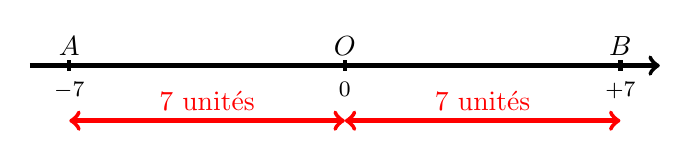
\begin{tikzpicture}
        % \draw[help lines, color=gray!30, dashed] (-4,-1) grid (4,.5);
        \draw[->,ultra thick] (-4,0)--(4,0);
        \draw[shift={(-3.5,0)},color=black,ultra thick] (0pt,2pt) -- (0pt,-2pt) node[below,fill=white] {\footnotesize $-7$};
        \draw (-3.5,0) node[above]{$A$};
        \draw[shift={(0,0)},color=black,ultra thick] (0pt,2pt) -- (0pt,-2pt) node[below,fill=white] {\footnotesize $0$};
        \draw (0,0) node[above]{$O$};
        \draw[shift={(3.5,0)},color=black,ultra thick] (0pt,2pt) -- (0pt,-2pt) node[below,fill=white] {\footnotesize $+7$};
        \draw (3.5,0) node[above]{$B$};
        \draw[<->,ultra thick,color=red] (-3.5,-.7)--(0,-.7);
        \draw (-1.75,-.7) node[above,color=red]{7 unités};
        \draw[<->,ultra thick,color=red] (0,-.7)--(3.5,-.7);
        \draw (1.75,-.7) node[above,color=red]{7 unités};
    \end{tikzpicture}

    $A$ et $B$ sont symétriques par rapport à $O$.
\end{exemple*1}

\begin{exemple*1}
    $\dfrac13$ et $-\dfrac13$ sont opposés.

    \begin{tikzpicture}
        \draw[help lines, color=gray!30, dashed] (-4,-1) grid (4,.5);
        \draw[->,ultra thick] (-4,0)--(4,0);
        \foreach \x in {-3,-2,...,3}
            \draw[shift={(\x,0)},color=black] (0pt,2pt) -- (0pt,-2pt);        
        \draw[shift={(3,0)},color=black,ultra thick] (0pt,2pt) -- (0pt,-2pt) node[below,fill=white] {\footnotesize $+1$};            
        \draw[shift={(-1,0)},color=black,ultra thick] (0pt,2pt) -- (0pt,-2pt) node[below,fill=white] {\footnotesize $-\dfrac13$};
        \draw (-1,0) node[above]{$C$};
        \draw[shift={(0,0)},color=black,ultra thick] (0pt,2pt) -- (0pt,-2pt) node[below,fill=white] {\footnotesize $0$};
        \draw (0,0) node[above]{$O$};
        \draw[shift={(1,0)},color=black,ultra thick] (0pt,2pt) -- (0pt,-2pt) node[below,fill=white] {\footnotesize $+\dfrac13$};
        \draw (1,0) node[above]{$D$};
        \draw[<->,ultra thick,color=red] (-1,-.9)--(0,-.9);
        % \draw (-.5,-.7) node[above,color=red]{1 tiers d'unités};
        \draw[<->,ultra thick,color=red] (0,-.9)--(1,-.9);
        % \draw (.5,-.7) node[above,color=red]{1 tiers d'7 unités};
    \end{tikzpicture}

    $C$ et $D$ sont symétriques par rapport à $O$.
\end{exemple*1}

\begin{propriete}[Soustraire un nombre relatif (admise)]
    Si on soustrait un nombre relatif alors cela revient à additionner son nombre opposé.
\end{propriete}

\begin{exemple*1}
    L'opposé de $+8,2$ est $-8,2$ et l'opposé de $+\dfrac34$ est $-\dfrac34$.
    \begin{itemize}
        \item Soustraire $+8,2$ revient à ajouter $-8,2$ d'où $(+14)-(+8,2)=(+14)+(-8,2)=+5,8$
        \item Soustraire $-8,2$ revient à ajouter $+8,2$ d'où $(-17,2)-(-8,2)=(-17,2)+(+8,2)=-9$
        \item Soustriare $+\dfrac34$ revient à ajouter $-\dfrac34$ d'où $\left(+\dfrac54\right) -\left(+\dfrac34\right)=\left(+\dfrac54\right) +\left(-\dfrac34\right)=\left(-\dfrac14\right)$
    \end{itemize}
\end{exemple*1}

% \begin{exemple*1}
%     répertoire

%     $\left(+\dfrac54\right) -\left(+\dfrac34\right)=\left(+\dfrac54\right) +\left(-\dfrac34\right)=\left(-\dfrac14\right)$
% \end{exemple*1}